\documentclass{article}
\usepackage[utf8]{inputenc}
\usepackage{tikz, pgfplots}
\usepackage[T1]{fontenc}
\usepackage{forest}
\usetikzlibrary{positioning, automata, calc}

%\usetikzlibrary{calc}

\title{Graphs Practices}
\begin{document}
\tableofcontents
\maketitle

\section{Practice Graph 1}
\vspace{50pt}
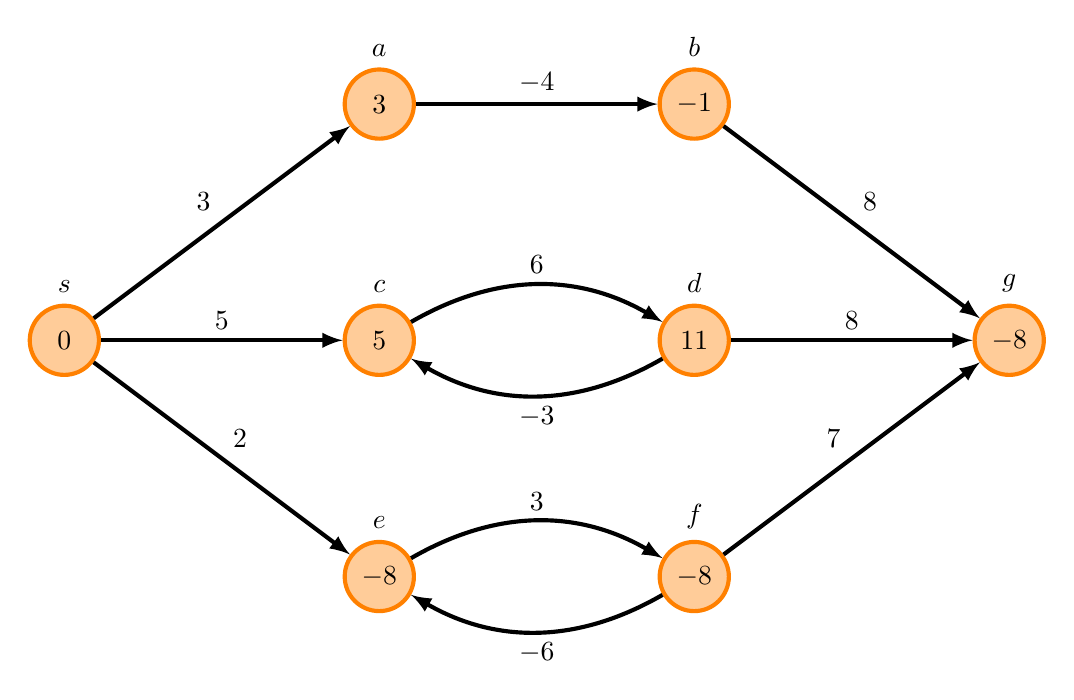
\begin{tikzpicture}[
    ->, 
    >=latex, % Use LaTeX-style arrows
    line width=1.5pt, % Increase the thickness of the arrow lines
    >=latex, scale=2, % Scale the arrowheads
    node distance=4cm and 0.2cm, % Adjust node distance (horizontal and vertical)
    auto % Automatically position labels
]

% Nodes with labels
\node[state,fill=orange!40,draw=orange ,label=above:{$\huge s$}] (A) {$0$};
\node[state,fill=orange!40,draw=orange , label=above:{$c$}] (B) [right of=A] {$5$};
\node[state,fill=orange!40,draw=orange , label=above:{$d$}] (C) [right of=B] {$11$};
\node[state,fill=orange!40,draw=orange , label=above:{$g$}] (D) [right of=C] {$-8$};

\node[state,fill=orange!40,draw=orange , label=above:{$a$}] (E) [above of=B,yshift=-1cm] {$3$};
\node[state, fill=orange!40,draw=orange ,label=above:{$b$}] (F) [above of=C,yshift=-1cm] {$-1$};

\node[state,fill=orange!40,draw=orange , label=above:{$e$}] (G) [below of=B,yshift=1cm] {$-8$};
\node[state, fill=orange!40,draw=orange ,label=above:{$f$}] (H) [below of=C,yshift=1cm] {$-8$};

% Edges with labels
\path (A) edge node {$5$} (B);
\path (B) edge[bend left] node {$6$} (C);
\path (C) edge[bend left] node {$-3$} (B);
\path (C) edge node {$8$} (D);

\path (A) edge node {$3$} (E);
\path (E) edge node {$-4$} (F);
\path (F) edge node {$8$} (D);

\path (A) edge node {$2$} (G);
\path (G) edge[bend left] node {$3$} (H);
\path (H) edge[bend left] node {$-6$} (G);
\path (H) edge node {$7$} (D);

\end{tikzpicture}

\section{Practice Graph 2(List)}
\vspace{50pt}
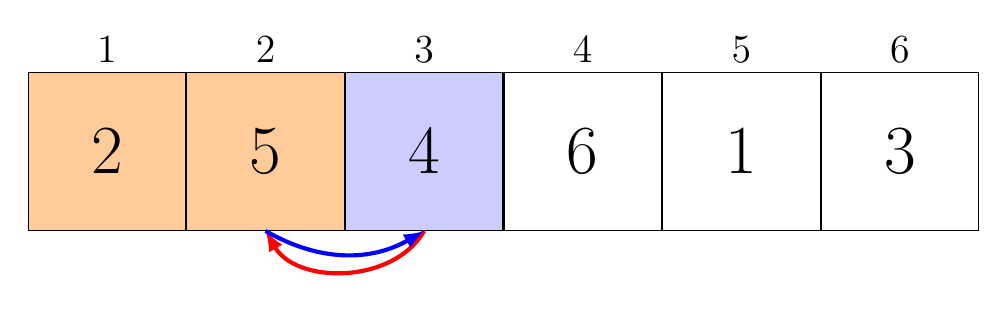
\begin{tikzpicture}[
    % Define a custom style for nodes
    mynode/.style={
        draw,
        rectangle,
        minimum width=2cm,
        minimum height=2cm
    }
]

% Define nodes using the custom style
\node[mynode,fill=orange!40,label=above:{\Large $1$}] (A) {\Huge 2};
\node[mynode, fill=orange!40,right=0pt of A,label=above:{\Large $2$}] (B) {\Huge 5};
\node[mynode,fill=blue!20, right=0pt of B,label=above:{\Large $3$}] (C) {\Huge 4};
\node[mynode, right=0pt of C,label=above:{\Large $4$}] (D) {\Huge 6};
\node[mynode, right=0pt of D,label=above:{\Large $5$}] (E) {\Huge 1};
\node[mynode, right=0pt of E,label=above:{\Large $6$}] (F) {\Huge 3};

% Edges with specific start and end points
\draw[red, line width=1.5pt, ->, >=latex, bend left=60] (C.south) to (B.south); % C to B with more bend
\draw[blue, line width=1.5pt, ->, >=latex,bend right=30] (B.south) to (C.south); % B to C with less bend

\end{tikzpicture}
\section{Practice graph 3 (linked list)}
\vspace{50pt}
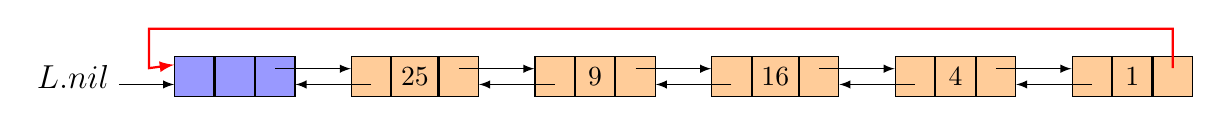
\begin{tikzpicture}[
% Define a custom style for nodes
    mynode/.style={
        draw,
        rectangle,
        minimum width=0.5cm,
        minimum height=0.5cm
        }
]
\node[fill=white] (S) {\large $L.nil$};

\node[mynode, fill=blue!40,right=20pt of S] (A) {};
\node[mynode, fill=blue!40,right=0pt of A] (B) {};
\node[mynode,fill=blue!40, right=0pt of B] (C) {};

\node[mynode, fill=orange!40,right=20pt of C] (D) {};
\node[mynode, fill=orange!40,right=0pt of D] (E) {$25$};
\node[mynode, fill=orange!40,right=0pt of E] (F) {};

\node[mynode, fill=orange!40,right=20pt of F] (G) {};
\node[mynode, fill=orange!40,right=0pt of G] (H) {$9$};
\node[mynode, fill=orange!40,right=0pt of H] (I) {};

\node[mynode, fill=orange!40,right=20pt of I] (J) {};
\node[mynode, fill=orange!40,right=0pt of J] (K) {$16$};
\node[mynode, fill=orange!40,right=0pt of K] (L) {};

\node[mynode, fill=orange!40,right=20pt of L] (M) {};
\node[mynode, fill=orange!40,right=0pt of M] (N) {$4$};
\node[mynode, fill=orange!40,right=0pt of N] (O) {};

\node[mynode, fill=orange!40,right=20pt of O] (P) {};
\node[mynode, fill=orange!40,right=0pt of P] (Q) {$1$};
\node[mynode, fill=orange!40,right=0pt of Q] (R) {};

\path[->,>=latex] ($(S.east) + (0, -0.1)$) edge node {} ($(A.west) + (0, -0.1)$);

\path[->,>=latex] ($(C.center) + (0, 0.1)$) edge node {} ($(D.west) + (0, 0.1)$);
\path[->,>=latex] ($(D.center) + (0, -0.1)$) edge node {} ($(C.east) + (0, -0.1)$);

\path[->,>=latex] ($(F.center) + (0, 0.1)$) edge node {} ($(G.west) + (0, 0.1)$);
\path[->,>=latex] ($(G.center) + (0, -0.1)$) edge node {} ($(F.east) + (0, -0.1)$);

\path[->,>=latex] ($(I.center) + (0, 0.1)$) edge node {} ($(J.west) + (0, 0.1)$);
\path[->,>=latex] ($(J.center) + (0, -0.1)$) edge node {} ($(I.east) + (0, -0.1)$);

\path[->,>=latex] ($(L.center) + (0, 0.1)$) edge node {} ($(M.west) + (0, 0.1)$);
\path[->,>=latex] ($(M.center) + (0, -0.1)$) edge node {} ($(L.east) + (0, -0.1)$);

\path[->,>=latex] ($(O.center) + (0, 0.1)$) edge node {} ($(P.west) + (0, 0.1)$);
\path[->,>=latex] ($(P.center) + (0, -0.1)$) edge node {} ($(O.east) + (0, -0.1)$);

\path[->,>=latex ,thick, draw=red]
    ($(R.north) + (0, -0.15)$) |- ++(0,0.5) -| ++(-13,0) |- ++(0,-0.5) -- ($(A.west) + (0,0.15)$);



\end{tikzpicture}

\section{Multiple trees}
\vspace{30pt}
\tikzset{
    treenode/.style={align=center, inner sep=0pt},
    node_orange/.style={treenode, circle, black, font=\bfseries, draw=orange, fill=orange!40, text width=0.5cm},
    node_blue/.style={treenode, circle, fill=blue!40, draw=blue, very thick, text width=0.5cm}
}

\begin{tabular}{cp{0.5cm}c}
\begin{tikzpicture}[->,  % Define sibling distances for each level
    level 1/.style={sibling distance=3cm},
    level 2/.style={sibling distance=2cm},
    level 3/.style={sibling distance=1cm},
    level distance=1.5cm % Vertical distance between levels
]
\node[node_orange]{16}
    child {node[node_blue,label = above:{2},label=left:{$i$}]{4}
        child {node[node_orange]{14}
            child {node[node_orange]{2}}
            child {node[node_orange]{8}}
        }
        child {node[node_orange]{7}
       		child {node[node_orange]{1}[shift={(-1em,0)}]}
        	child[missing]
        }
    }
    child {node[node_blue]{10}
        child{node[node_orange]{9}}
        child {node[node_orange]{3}}
    };

\end{tikzpicture}

&
&\begin{tikzpicture}[->,  % Define sibling distances for each level
    level 1/.style={sibling distance=3cm},
    level 2/.style={sibling distance=2cm},
    level 3/.style={sibling distance=1cm},
    level distance=1.5cm % Vertical distance between levels
]
\node[node_orange]{16}
    child {node[node_blue]{4}
        child {node[node_orange]{14}
            child {node[node_orange]{2}}
            child {node[node_orange]{8}}
        }
        child {node[node_orange]{7}
            child{node[node_orange]{1}}
            child[missing]
        }
    }
    child {node[node_blue]{10}
        child{node[node_orange]{9}}
        child {node[node_orange]{3}}
    };
    
\end{tikzpicture}
\end{tabular}

\section{Dashed tree}
\vspace{30pt}
\tikzset{
    treenode/.style={align=center, inner sep=0pt},
    node_white/.style={treenode, circle, black, font=\bfseries, draw=white, fill=white, text width=0.5cm},
    small-dashed/.style={-, dashed, dash pattern=on 2pt off 2pt, thick, draw=black}, % Custom small dashed line style
}

\begin{tikzpicture}[
    level 1/.style={sibling distance=6cm},
    level 2/.style={sibling distance=3cm},
    level 3/.style={sibling distance=1cm},
    level 4/.style={sibling distance=0.5cm},
    level distance=3cm,
    edge from parent/.style={-, dashed, dash pattern=on 2pt off 2pt, thick, draw=black} % Apply small dashed style globally
]
\node[node_white]{$c_2n$}
    child {node[node_white]{$c_2n/2$}
        child {node[node_white]{$c_2n/4$}
            child {node[node_white]{$c_1$}}
            child {node[node_white]{$c_1$}}
            child {node[node_white]{$c_1$}} 
        }
        child[missing]
        child {node[node_white]{$c_2n/4$}}  
    }
    child {node[node_white]{$c_2n/2$}
        child {node[node_white]{$c_2n/4$}} 
        child {node[node_white]{$c_2n/4$}} 
    };

\end{tikzpicture}


\end{document}
